% Options for packages loaded elsewhere
\PassOptionsToPackage{unicode}{hyperref}
\PassOptionsToPackage{hyphens}{url}
%
\documentclass[
  spanish,
  ignorenonframetext,
]{beamer}
\usepackage{pgfpages}
\setbeamertemplate{caption}[numbered]
\setbeamertemplate{caption label separator}{: }
\setbeamercolor{caption name}{fg=normal text.fg}
\beamertemplatenavigationsymbolsempty
% Prevent slide breaks in the middle of a paragraph
\widowpenalties 1 10000
\raggedbottom
\setbeamertemplate{part page}{
  \centering
  \begin{beamercolorbox}[sep=16pt,center]{part title}
    \usebeamerfont{part title}\insertpart\par
  \end{beamercolorbox}
}
\setbeamertemplate{section page}{
  \centering
  \begin{beamercolorbox}[sep=12pt,center]{part title}
    \usebeamerfont{section title}\insertsection\par
  \end{beamercolorbox}
}
\setbeamertemplate{subsection page}{
  \centering
  \begin{beamercolorbox}[sep=8pt,center]{part title}
    \usebeamerfont{subsection title}\insertsubsection\par
  \end{beamercolorbox}
}
\AtBeginPart{
  \frame{\partpage}
}
\AtBeginSection{
  \ifbibliography
  \else
    \frame{\sectionpage}
  \fi
}
\AtBeginSubsection{
  \frame{\subsectionpage}
}
\usepackage{amsmath,amssymb}
\usepackage{lmodern}
\usepackage{ifxetex,ifluatex}
\ifnum 0\ifxetex 1\fi\ifluatex 1\fi=0 % if pdftex
  \usepackage[T1]{fontenc}
  \usepackage[utf8]{inputenc}
  \usepackage{textcomp} % provide euro and other symbols
\else % if luatex or xetex
  \usepackage{unicode-math}
  \defaultfontfeatures{Scale=MatchLowercase}
  \defaultfontfeatures[\rmfamily]{Ligatures=TeX,Scale=1}
\fi
\usetheme[]{Darmstadt}
\usecolortheme{seahorse}
\usefonttheme{structurebold}
% Use upquote if available, for straight quotes in verbatim environments
\IfFileExists{upquote.sty}{\usepackage{upquote}}{}
\IfFileExists{microtype.sty}{% use microtype if available
  \usepackage[]{microtype}
  \UseMicrotypeSet[protrusion]{basicmath} % disable protrusion for tt fonts
}{}
\makeatletter
\@ifundefined{KOMAClassName}{% if non-KOMA class
  \IfFileExists{parskip.sty}{%
    \usepackage{parskip}
  }{% else
    \setlength{\parindent}{0pt}
    \setlength{\parskip}{6pt plus 2pt minus 1pt}}
}{% if KOMA class
  \KOMAoptions{parskip=half}}
\makeatother
\usepackage{xcolor}
\IfFileExists{xurl.sty}{\usepackage{xurl}}{} % add URL line breaks if available
\IfFileExists{bookmark.sty}{\usepackage{bookmark}}{\usepackage{hyperref}}
\hypersetup{
  pdftitle={Clase 3: Los Nomencladores de clases sociales},
  pdfauthor={Nicolás Sacco; José Rodríguez de la Fuente; Sofia Jaime},
  pdflang={es},
  hidelinks,
  pdfcreator={LaTeX via pandoc}}
\urlstyle{same} % disable monospaced font for URLs
\newif\ifbibliography
\usepackage{longtable,booktabs,array}
\usepackage{calc} % for calculating minipage widths
\usepackage{caption}
% Make caption package work with longtable
\makeatletter
\def\fnum@table{\tablename~\thetable}
\makeatother
\setlength{\emergencystretch}{3em} % prevent overfull lines
\providecommand{\tightlist}{%
  \setlength{\itemsep}{0pt}\setlength{\parskip}{0pt}}
\setcounter{secnumdepth}{-\maxdimen} % remove section numbering
\ifxetex
  % Load polyglossia as late as possible: uses bidi with RTL langages (e.g. Hebrew, Arabic)
  \usepackage{polyglossia}
  \setmainlanguage[]{spanish}
\else
  \usepackage[main=spanish]{babel}
% get rid of language-specific shorthands (see #6817):
\let\LanguageShortHands\languageshorthands
\def\languageshorthands#1{}
\fi
\ifluatex
  \usepackage{selnolig}  % disable illegal ligatures
\fi

\title{Clase 3: Los Nomencladores de clases sociales}
\author{Nicolás Sacco \and José Rodríguez de la Fuente \and Sofia Jaime}
\date{2021-10-25}
\institute{Taller de Análisis de la Estructura Social en la Argentina
Contemporánea Maestría en Generación y Análisis de Información
Estadística (UNTREF)}

\begin{document}
\frame{\titlepage}

\hypertarget{presentaciuxf3n-de-la-clase}{%
\section{Presentación de la clase}\label{presentaciuxf3n-de-la-clase}}

\begin{frame}{Contenidos}
\protect\hypertarget{contenidos}{}
En esta clase se realiza un recorrido por los siguientes contenidos:

\begin{enumerate}
\tightlist
\item
  Operacionalización del concepto de clase social\\
\item
  Enfoques empíricos de clases sociales\\
\item
  Operacionalización paso a paso
\item
  Operacionalización automática\\
\item
  Unidades de análisis\\
\item
  Operadores relacionales y lógicos
\end{enumerate}
\end{frame}

\hypertarget{las-clases-en-la-computadora}{%
\section{Las clases en la
computadora}\label{las-clases-en-la-computadora}}

\begin{frame}{Operacionalizando el concepto de clase}
\protect\hypertarget{operacionalizando-el-concepto-de-clase}{}
\begin{itemize}
\tightlist
\item
  Operacionalización: pasaje de conceptos teórico-abstractos a
  indicadores empíricos\\
\item
  Las clases sociales son una parte de la \textbf{estructura social}

  \begin{itemize}
  \tightlist
  \item
    El proceso de operacionalización nos permite separarla del resto de
    las dimensiones
  \end{itemize}
\end{itemize}
\end{frame}

\begin{frame}{¿Clases, grupos o estratos?}
\protect\hypertarget{clases-grupos-o-estratos}{}
\begin{itemize}
\tightlist
\item
  Ambigüedad de los conceptos\\
\item
  Cada concepto corresponde a una tradición teórica\\
\item
  Criterios para la construcción de clasificaciones:

  \begin{itemize}
  \tightlist
  \item
    \emph{Elección de medidas}: medidas continuas o categóricas\\
  \item
    \emph{Naturaleza de la información}: subjetiva u objetiva\\
  \item
    \emph{Objeto de la medición}: estatus, clases, prestigio, etc.
  \end{itemize}
\end{itemize}
\end{frame}

\hypertarget{enfoques-empuxedricos-de-clases}{%
\section{Enfoques empíricos de
clases}\label{enfoques-empuxedricos-de-clases}}

\begin{frame}{Enfoque EGP}
\protect\hypertarget{enfoque-egp}{}
\begin{figure}

{\centering 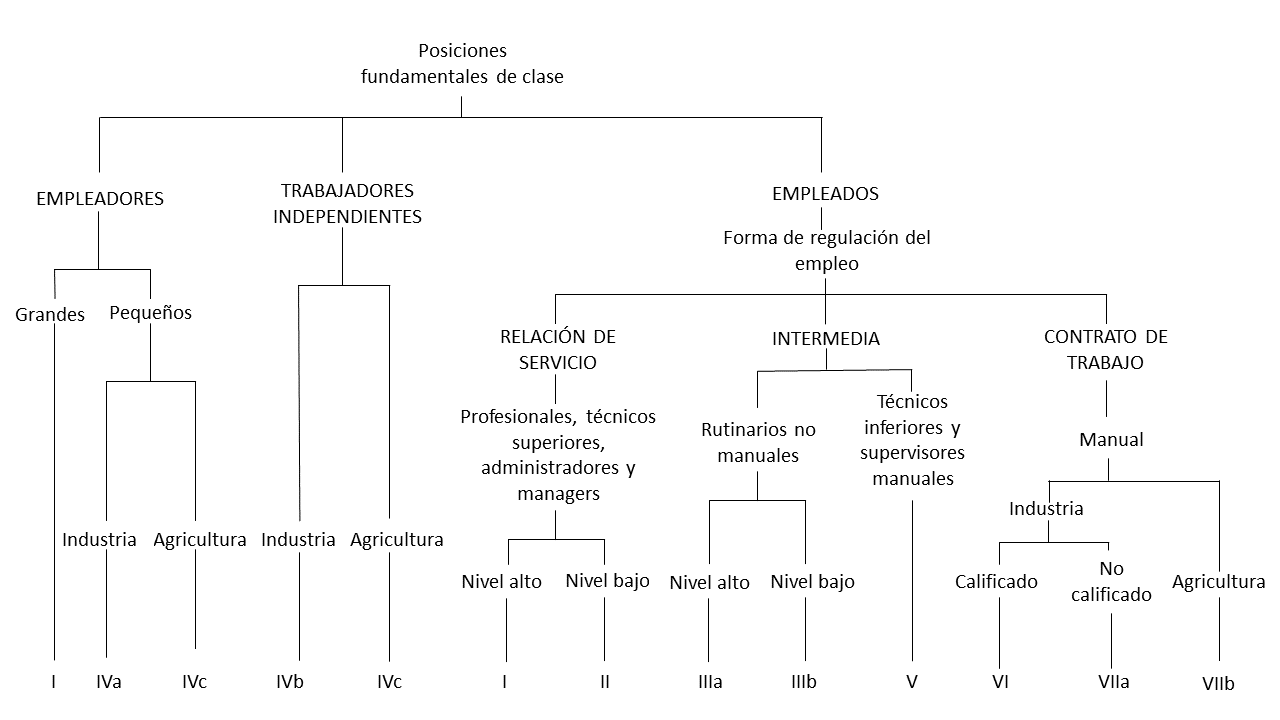
\includegraphics[width=0.85\linewidth]{imagenes/esquema_egp} 

}

\caption{Derivación del esquema de clases EGP. Fuente: Erikson y Goldthorpe (1992)}\label{fig:unnamed-chunk-1}
\end{figure}
\end{frame}

\begin{frame}{Enfoque Wright}
\protect\hypertarget{enfoque-wright}{}
\begin{figure}

{\centering 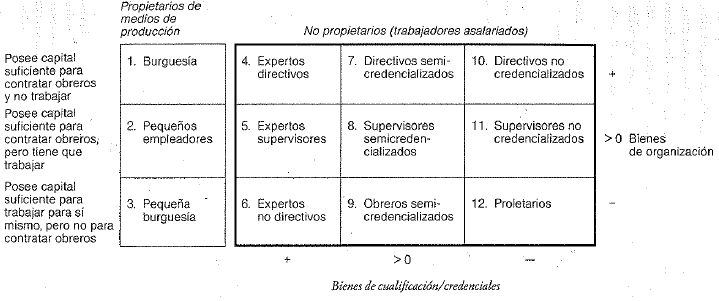
\includegraphics[width=0.85\linewidth]{imagenes/wright1} 

}

\caption{Tipología de las posiciones de clase en la sociedad capitalista. Wright (1994)}\label{fig:unnamed-chunk-2}
\end{figure}
\end{frame}

\begin{frame}{Enfoques gradacionales - Escala SIOPS}
\protect\hypertarget{enfoques-gradacionales---escala-siops}{}
\begin{figure}

{\centering 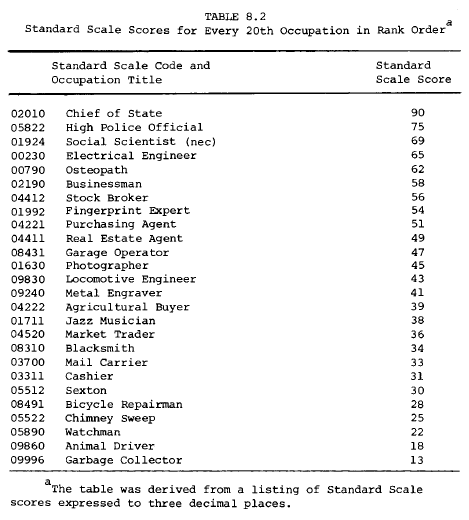
\includegraphics[width=0.5\linewidth]{imagenes/treiman} 

}

\caption{Puntajes estandard ordenados de 20 ocupaciones seleccionadas a partir de la escala SIOPS. Treiman(1977)}\label{fig:unnamed-chunk-3}
\end{figure}
\end{frame}

\begin{frame}{Enfoques gradacionales - Escala ISEI}
\protect\hypertarget{enfoques-gradacionales---escala-isei}{}
\begin{figure}

{\centering 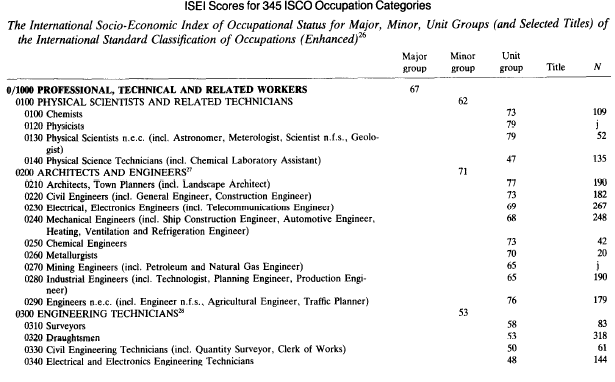
\includegraphics[width=0.85\linewidth]{imagenes/isei} 

}

\caption{Puntajes del ISEI de las primeras ocupaciones de la CIUO. Ganzeboom, Treiman y de Graaf (1992)}\label{fig:unnamed-chunk-4}
\end{figure}
\end{frame}

\begin{frame}{Enfoques nacionales - Germani}
\protect\hypertarget{enfoques-nacionales---germani}{}
\begin{figure}

{\centering 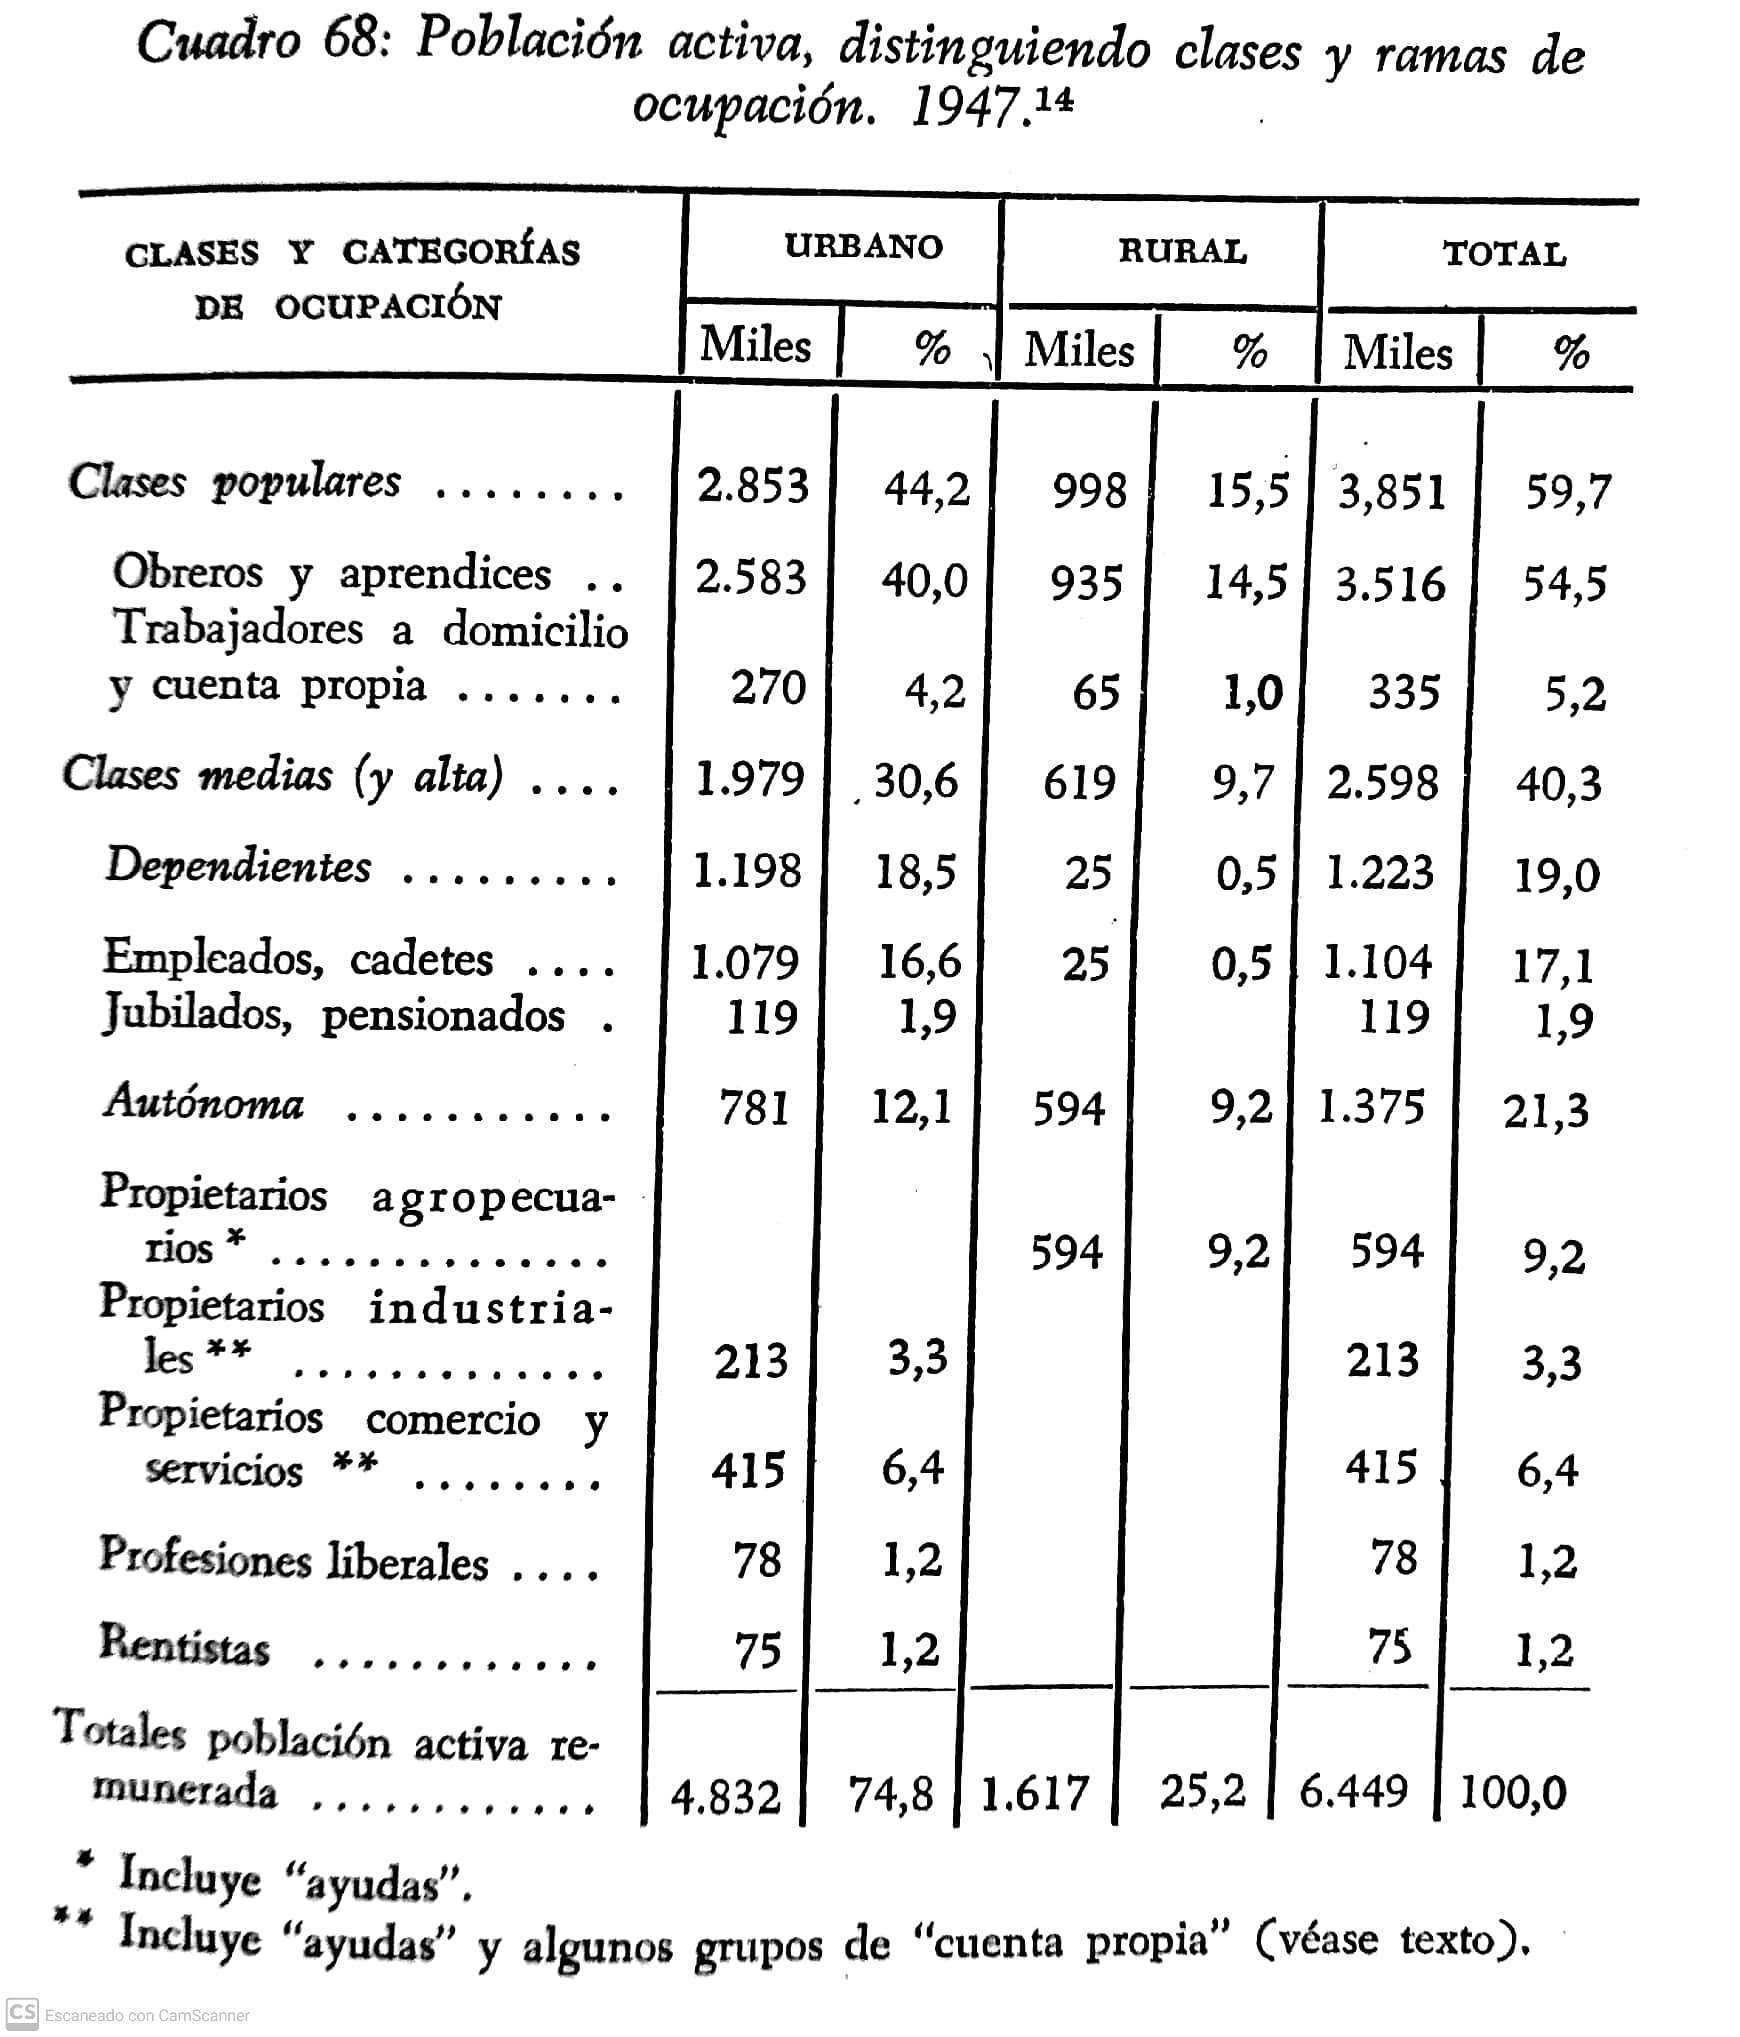
\includegraphics[width=0.5\linewidth]{imagenes/germani} 

}

\caption{Esquema de clases de Gino Germani (Germani, 1955)}\label{fig:unnamed-chunk-5}
\end{figure}
\end{frame}

\begin{frame}{Enfoques nacionales - Torrado}
\protect\hypertarget{enfoques-nacionales---torrado}{}
\begin{figure}

{\centering 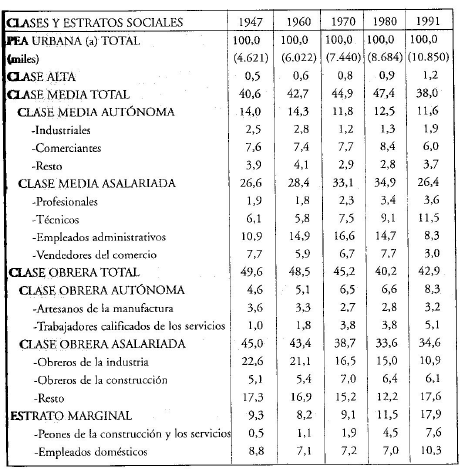
\includegraphics[width=0.55\linewidth]{imagenes/torrado4} 

}

\caption{Evolución de la estructura de clases. Total país 1947-1991. Torrado (2007)}\label{fig:unnamed-chunk-6}
\end{figure}
\end{frame}

\hypertarget{unidades-de-anuxe1lisis}{%
\section{Unidades de análisis}\label{unidades-de-anuxe1lisis}}

\begin{frame}{Discusión teórica - metodológica}
\protect\hypertarget{discusiuxf3n-teuxf3rica---metodoluxf3gica}{}
\begin{itemize}
\tightlist
\item
  Siempre debe basarse en el marco teórico y los objetivos de la
  investigación\\
\item
  ¿Población ocupada, PEA o población total?\\
\item
  ¿Individuos u hogares?\\
\item
  Enfoques para el estudio de los hogares

  \begin{enumerate}
  \tightlist
  \item
    Tradicional: jefe/a de hogar\\
  \item
    Dominancia: el cónyuge de mayor nivel ocupacional define la clase
    del hogar\\
  \item
    Clases híbridas: posición de ambos cónyuges
  \end{enumerate}
\end{itemize}
\end{frame}

\hypertarget{operadores}{%
\section{Operadores}\label{operadores}}

\begin{frame}{Operadores relacionales}
\protect\hypertarget{operadores-relacionales}{}
\begin{itemize}
\tightlist
\item
  Permiten relacionar a los valores asumidos en un variable con un valor
  de referencia\\
\item
  Siempre que estén bien formulados devuelven un resultado lógico
  (verdadero o falso)\\
\item
  No pueden utilizarse con variables de tipo \emph{cadena}\\
\item
  Tipos de operadores relacionales:
\end{itemize}

\begin{longtable}[]{@{}llll@{}}
\toprule
Operador & Comparación & Ejemplo & Resultado \\
\midrule
\endhead
\textless{} & Menor que & 4 \textless{} 1 & FALSO \\
\textless= & Menor o igual que & 4 \textless= 1 & FALSO \\
\textgreater{} & Mayor que & 8 \textgreater{} 6 & VERDADERO \\
\textgreater= & Mayor o igual que & 8 \textgreater= 6 & VERDADERO \\
== & Exactamente igual que & 7 == 9 & FALSO \\
!= & No es igual que & 5 != 2 & VERDADERO \\
\bottomrule
\end{longtable}
\end{frame}

\begin{frame}{Operadores lógicos}
\protect\hypertarget{operadores-luxf3gicos}{}
\begin{itemize}
\tightlist
\item
  También llamados operadores \emph{booleanos}\\
\item
  Permiten vincular proposiciones construidas a partir de operadores
  relacionales\\
\item
  Nos van a permiter crear relaciones complejas\\
\item
  Tipos de operadores lógicos:
\end{itemize}

\begin{longtable}[]{@{}llll@{}}
\toprule
Operador & Comparación & Ejemplo & Resultado \\
\midrule
\endhead
x \textbar{} y & x Ó y es verdadero & V \textbar{} F & VERDADERO \\
x \& y & x Y y son verdaderos & V \& F & FALSO \\
!x & x no es verdadero (negación) & !v & FALSO \\
\bottomrule
\end{longtable}
\end{frame}

\end{document}
